
    \documentclass{article}

    %  Русский язык

    \usepackage[T2A]{fontenc}			% кодировка
    \usepackage[utf8]{inputenc}			% кодировка исходного текста
    \usepackage[english,russian]{babel}	% локализация и переносы
    \usepackage{unicode-math}

    % Рисунки
    \usepackage{graphicx, float}
    \usepackage{wrapfig}


    \title{Wild wild west derivative counter}
    \author{Dodo}
    \date{November 2022}


    \begin{document}
    \maketitle
    
        Welcome to derivative calculator fella, let's have a look at ya. God, what da hell is dis shit, fella?
        Ok, ok, let's calculate this bullshit.

        \begin{center}
        $\clubsuit$~$\clubsuit$~$\clubsuit$
        \end{center}
    Got to calculate function in point 5
The result is 0\begin{center} $\clubsuit$~$\clubsuit$~$\clubsuit$ \end{center}\begin{figure}[H] 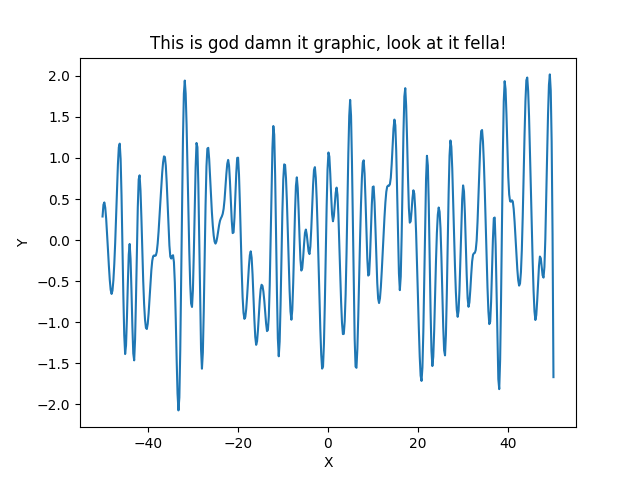
\includegraphics[scale=0.6]{function_graph.png} \end{figure}Alright fella, let's look wat we got:

\begin{equation}
{ln({\frac{({sin({X})})}{({cos({{{2}\cdot{X}}-{5}})})}})}
\end{equation}
\begin{center} $\clubsuit$~$\clubsuit$~$\clubsuit$ \end{center}With the power of gods, let's write the following:
\begin{equation}
{ln({\frac{({sin({X})})}{({cos({{{2}\cdot{X}}-{5}})})}})}
\end{equation}
\begin{center} $\clubsuit$~$\clubsuit$~$\clubsuit$ \end{center}I smacked a damn big cockroach yesterday fella, this was left on my shoe:
\begin{equation}
{\frac{({sin({X})})}{({cos({{{2}\cdot{X}}-{5}})})}}
\end{equation}
\begin{center} $\clubsuit$~$\clubsuit$~$\clubsuit$ \end{center}Don't distract fella, I don't know how to count
\begin{equation}
{cos({{{2}\cdot{X}}-{5}})}
\end{equation}
\begin{center} $\clubsuit$~$\clubsuit$~$\clubsuit$ \end{center}Oh come on, my wife is pregnant 12th time in a row.
\begin{equation}
{{{2}\cdot{X}}-{5}}
\end{equation}
\begin{center} $\clubsuit$~$\clubsuit$~$\clubsuit$ \end{center}Can you understand it by yourself, i must go get some beer, fella:
\begin{equation}
{{2}\cdot{X}}
\end{equation}
\begin{center} $\clubsuit$~$\clubsuit$~$\clubsuit$ \end{center}...
\begin{equation}
{sin({X})}
\end{equation}
\begin{center} $\clubsuit$~$\clubsuit$~$\clubsuit$ \end{center}Here is whach you got, fella. Now let's drink some whiskey and shoot niggers.
\begin{equation}
{({\frac{({1})}{({\frac{({sin({X})})}{({cos({{{2}\cdot{X}}-{5}})})}})}})\cdot({\frac{({{({({cos({X})})\cdot({1})})\cdot({cos({{{2}\cdot{X}}-{5}})})}-{({sin({X})})\cdot({({({-1})\cdot({sin({{{2}\cdot{X}}-{5}})})})\cdot({{2}-{0}})})}})}{({({cos({{{2}\cdot{X}}-{5}})})\cdot({cos({{{2}\cdot{X}}-{5}})})})}})}
\end{equation}
\begin{center} $\clubsuit$~$\clubsuit$~$\clubsuit$ \end{center}
        The solution is pretty simple and you definetely can do it \textbf{yourself}
        \end{document}
    